\section{Evaluation} 
\label{sec:eval}

\begin{figure*}[!t]
    \centering
    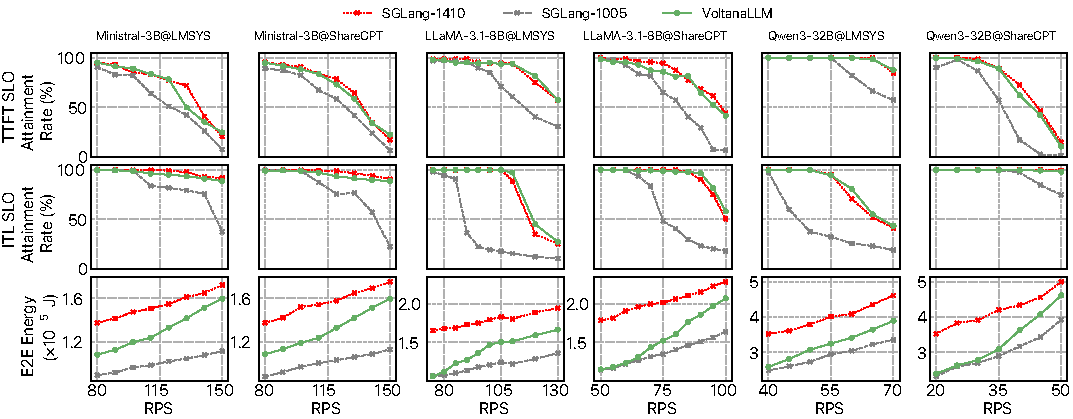
\includegraphics[width=\linewidth]{figs/main_result_combined.pdf}
    \caption{The TTFT/ITL SLO attainment rates and E2E energy consumption comparing \name and baselines across diverse models and datasets. \name consistently maintains latency SLO attainment rates comparable or slightly better than SGLang-1410, while significantly reducing E2E energy consumption.}
    \vspace{-1em}
    \label{fig:main-result}
\end{figure*}

\subsection{Evaluation Methodology}
\label{subsec:eval-method}

\noindent
\textbf{Implementation.}
We implement \name in Python on top of SGLang (v0.4.7.post1)~\cite{zheng2024sglang}, a widely used LLM inference framework with production-level P/D disaggregation support.
As described in \sref{subsec:governor}, \governor runs in a separate process to overlap overhead, and pyNVML~\cite{pynvml} is used for minimal-overhead frequency setting. 
\appref{subsubssec:xgboost} details the XGBoost model configurations of \predictor.

\noindent
\noindent
\textbf{Models and Workloads.}
We evaluate \name on Ministral-3B~\cite{ministral}, LLaMA-3.1-8B~\cite{grattafiori2024llama}, and Qwen3-32B~\cite{yang2025qwen3} using ShareGPT~\cite{sharegpt} and LMSYS-Chat-1M~\cite{zheng2023lmsys} workloads (more details in \appref{appendix:dataset-length}) with Poisson-distributed controlled request arrival rates (\emph{Requests-Per-Second}, RPS).

\noindent
\textbf{Metrics.}
We measure performance via TTFT, ITL, and the SLO attainment rate.
\cameraready{
Following DistServe~\cite{zhong2024distserve}, SLO is defined as the target upper bounds of TTFT or ITL, and attainment rate refers to the percentage of requests satisfying these bounds ($\text{TTFT}\le S_P$, $\text{ITL}\le S_D$).}
We report end-to-end energy consumption (Joules) measured via pyNVML.

\noindent
\textbf{Hardware Testbeds.} All experiments are performed on NVIDIA A100-80G SXM4 GPUs connected via NVLink.



\subsection{Main Result}
\label{subsec:main-result}


We evaluate \name across all models and datasets, using a 2P2D (2 prefill and 2 decode instances) configuration. 
For Qwen3-32B, 2-way Tensor Parallelism~\cite{shoeybi2019megatron} is used for each instance.
The frequency options of \governor are set to $\mathcal{F}=\{1005, 1410\}$ MHz, and the imbalance prevention threshold of \router is set to $\Delta=500$, which allows both frequencies to co-exist for different instances.
TTFT/ITL SLOs are set to 200/20, 600/60, 1200/120 ms for Ministral-3B, LLaMA-3.1-8B, and Qwen3-32B, respectively.
While DynamoLLM~\cite{stojkovic2025dynamollm} and throttLL’eM~\cite{kakolyris2025throttll} are the most relevant systems to our work, they are not included for comparison due to the lack of publicly available code.
As such, we construct two baselines based on SGLang:
\textbf{SGLang-1005}, using a static 1005 MHz frequency (the ``sweet spot'' described in \sref{sec:obs-u-shape}), and \textbf{SGLang-1410}, using the static maximum frequency (1410 MHz, the default strategy of A100~\cite{vspetko2021dgx}).
These baselines use SGLang's default round-robin request routing.
For each configuration, we report: (1) TTFT SLO attainment rate, (2) ITL SLO attainment rate, and (3) E2E energy consumption.


\fref{fig:main-result} shows our results, from which we have two key findings.
First, \name consistently achieves comparable TTFT SLO attainment rates and comparable or slightly better ITL SLO attainment rate compared to SGLang-1410, which operates at the static maximum frequency.
It significantly outperforms  SGLang-1005, which is energy efficient but yields substantially lower SLO attainment.
This ability to maintain high SLO attainment is attributed to the SLO-aware design of \governor.
It adaptively selects the GPU frequency for each engine iteration to ensure the model inference time remains within the budget.
Notably, the slightly better ITL SLO attainment compared to SGLang-1410 in some situations is attributed to \router.
As illustrated in \fref{fig:router-motivation}, \router allows one instance to avoid crossing a batch size boundary and frequency ``cliff'', at the cost of a marginal ITL increase in another instance.
This increase is outweighed by the ITL reduction benefit from avoiding the boundary.
Second, while preserving latency SLOs, \name reduces E2E energy consumption by up to 36.3\% compared to SGLang-1410.
\cameraready{The peak energy reduction occurs under the specific configuration of Qwen3-32B with ShareGPT at RPS of 20.}
Its effectiveness is most pronounced at low request rates, where a static low frequency is sufficient for SLO targets, so \name dynamically operates at a low frequency most of the time.
Conversely, at high request rates, it dynamically increases frequency to maintain SLO attainment, resulting in smaller yet still significant energy benefits.

We also provide the throughput metrics in \appref{subsubsec:ablation-throughput} and latency Cumulative Distribution Functions (CDFs) in \appref{subsubssec:main-cdf} for more details.
\cameraready{
\appref{subsubsec:intermidate-static-freq} provides a comparison between \name and SGLang using additional intermediate static frequencies beyond 1005 and 1410~MHz, while \appref{subsubsec:power-capped} provides a comparison against power-capped SGLang baselines. 
Both static and power-capped baselines inherently lack adaptability to workload dynamism, failing to achieve energy savings and SLO attainment comparable to \name. 
Furthermore, \appref{subsubsec:phase-specific-energy-gain} provides a detailed breakdown of the phase-specific energy savings achieved by \name.
}
For configuration with multiple levels of frequency options in \governor, we provide results and comparison in \appref{subsubsec:exp-multi-level}.
\cameraready{
Additionally, \appref{subsubsec:delta-analysis} presents a sensitivity analysis of $\Delta$ in \router, demonstrating that a larger $\Delta$ has a slight negative impact on ITL SLO attainment for \name under multi-level frequency settings.
}


Overall, these improvements validate that SLO-aware frequency control and request routing effectively optimize energy consumption while preserving the quality of service. 






\subsection{Analysis Results}
\label{subsec:analysis}


\noindent
\textbf{How does each module of \name bring benefits?}
To quantify the per-component contribution in \name, we conduct experiments similar to \sref{subsec:main-result} using the ShareGPT dataset and LLaMA-3.1-8B model, but with two additional system configurations: \textbf{\governor-only} and a full version of \textbf{\name} (\governor+ \router).
\fref{fig:sys-design-each-module} presents the results.
First, \governor-only achieves substantial energy savings for both prefill and decode instances compared to the static high-frequency baseline SGLang-1410, validating the effectiveness of its SLO-aware frequency control policy.
\fref{fig:freq-time} provides an example of real-time frequency traces.
At low request rates, both P/D instances mainly operate at low frequency to conserve energy, while the proportion of high-frequency time increases for higher request rates due to SLO targets.
Second, the full \name achieves additional energy reductions compared to \governor-only, which is decode specific as \router is only applied to the decode instances.
\appref{subsubsec:router-example} gives an example to compares round-robin and \router by the frequencies of the two decode instances over time.
It shows \router can restrict the batch size of one instance under a specific boundary (256) so it can operate at a lower frequency.
% \jiahuan{\fref{fig:bs-time} is the candidate to move to appendix}



\begin{figure}[!t]
    \centering
    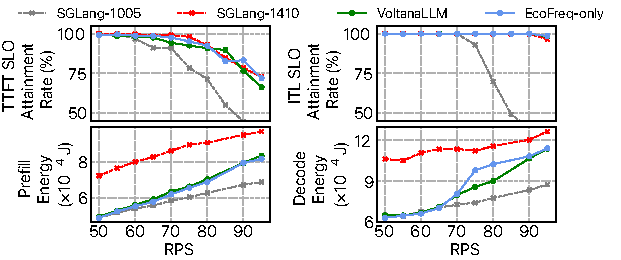
\includegraphics[width=\columnwidth]{figs/ablation_w_router-2p2d.pdf}
    \caption{Comparison of \governor-only and full \name. \governor-only reduces energy for both prefill and decode while preserving SLOs, and 
    \router yields additional energy savings for the decode phase.} % by avoiding high-frequency regions.}
    % \jiahuan{@Junfeng, change the y axis label of 2nd row to 3 lines}
   
    \label{fig:sys-design-each-module}
\end{figure}

\begin{figure}[!t]
    \centering
    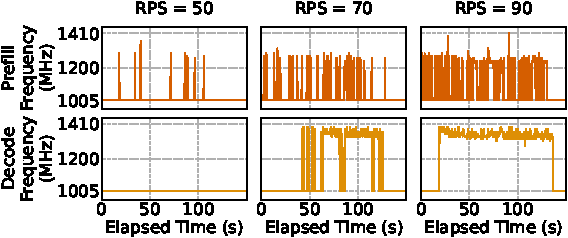
\includegraphics[width=0.95\columnwidth]{figs/ablation-freq-time-combined.pdf}
    \caption{Real-time frequency traces of \governor-only for P/D instances at different request rates. At low RPS, instances primarily operate at low frequency, As RPS increases, both shift to high frequency more often.} % to maintain SLOs.}
    \label{fig:freq-time}
\end{figure}



\noindent
\textbf{How does \name perform under different latency SLO targets?}
We evaluate \name on LLaMA-3.1-8B with the ShareGPT dataset, following the settings in \sref{subsec:main-result} but testing three different TTFT/ITL SLO profiles: 400/40 (``low''), 600/60 (``medium''), and 800/80 (``high'').
\fref{fig:slo-sensitivity} presents the results.
Across all SLO profiles, \name consistently achieves SLO attainment rates comparable or slightly better than the static maximum frequency baseline.
Specifically, as the SLO constraints are relaxed (i.e., from ``low'' to ``high''), \name's adaptive frequency control trades higher latency for lower energy consumption.
This demonstrates the latency-energy trade-off, providing the flexibility to define custom scenario and phase-specific SLOs, such as prioritizing low ITL for responsiveness or low energy consumption to reduce cost.
This result further emphasizes the necessity of the phase-specific design as discussed in \sref{sec:observations}.







% \begin{figure}[!t]
%     \centering
%     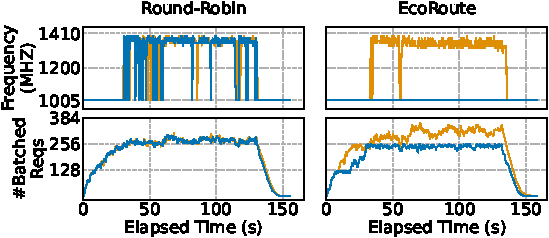
\includegraphics[width=\columnwidth]{figs/ablation-router.pdf}
%     \caption{An example of how \router differs from round-robin policy (RPS=75). Each line represents a decode instance. \router keeps one instance below the batch size boundary (256), allowing it to run at a lower frequency for longer time. }    
%     % \minjia{Candidate move to the appendix.}
%     % \jiahuan{if we decide to remove this figure from here, can we replace \fref{fig:router-example} with this figure. \fref{fig:router-example} is just a conceptual version of it.}
%     % \minjia{Yes, although I would try to avoid adding too many empirical results in the design. }
%     \label{fig:bs-time}
% \end{figure}


\begin{figure}[!t]
    \centering
    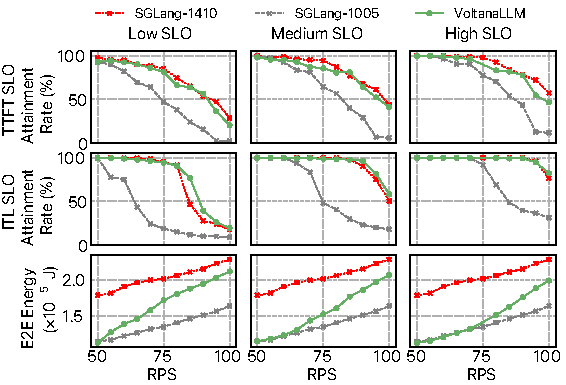
\includegraphics[width=0.95\columnwidth]{figs/ablation-slo.pdf}
    \caption{Comparison of \name and baselines under different SLO profiles (low, medium, high).
    Across all settings, \name maintains strong TTFT and ITL SLO attainment rates while providing significant energy savings.}
    \label{fig:slo-sensitivity}
\end{figure}

\noindent
\textbf{How important is it to have per-iteration frequency control?}
In \sref{subsec:temporal-variation}, we show rapid iteration-level workload variation in LLM serving, which necessitates the design for per-iteration frequency control.
\name provides this iteration-level responsiveness, unlike prior approaches~\cite{stojkovic2025dynamollm} that adjust frequency at coarser, window-based intervals (e.g., 5s).
To verify its benefit, we adapt \governor to operate at various fixed time intervals, evaluating it using the ShareGPT dataset on LLaMA-3.1-8B under the 1P1D configuration (where \router has no effect).
The results in \fref{fig:time-window} demonstrate that window-based frequency control degrades SLO attainment for both phases.
Specifically, per-iteration frequency responsiveness is particularly critical for the prefill phase, where window-based control shows larger degradation.
Due to dynamic batching, the total number of tokens processed in a prefill batch (and thus the optimal frequency) can vary significantly from one iteration to the next, as \fref{fig:prefill-tokens-fluctuation} shows.
A window-based approach is too coarse-grained to react to such rapid changes.
In contrast, as shown in \fref{fig:bs-time}, the load of the decode instance shows smoother change in batched requests, leading to relative insensitivity to window interval settings.

\begin{figure}[!t]
    \centering
    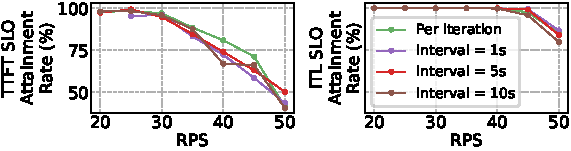
\includegraphics[width=0.95\columnwidth]{figs/ablation-interval.pdf}
    \caption{Latency SLO attainment rates across different frequency control intervals. Our per-iteration design provides the best responsiveness, and thereby the highest SLO attainment rates.}
    \label{fig:time-window}
\end{figure}


\noindent
\textbf{Is \predictor accurate? Can online adaptation improve accuracy?}
To verify these aspects, we compare \predictor's predicted values against the empirical latency results from \sref{subsec:main-result}, evaluating both the initial offline-trained and the online-adapted models.
\fref{fig:pred-accuracy} shows the results.
Both TTFT and ITL predictions consistently achieve low mean absolute errors (MAEs) across all models, which enables the SLO-aware frequency selection of \governor.
Furthermore, online adaptation provides a clear MAE improvement, which successfully mitigates the sample distribution shift (\fref{fig:dist-shift}).


% \minjia{TODO: May need one figure to show how the model's online adapation performs. }
% \jiahuan{done}

\begin{figure}[!t]
    \centering
    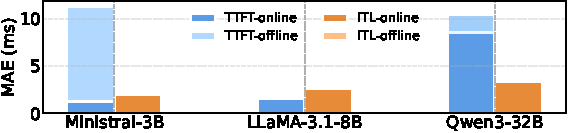
\includegraphics[width=0.85\columnwidth]{figs/prediction_error.pdf}
    \caption{Mean absolute errors (MAEs) of \predictor for both TTFT and ITL, comparing the offline-only model to the online-adapted model.} % across all evaluated models.}
    % \jiahuan{@Junfeng, squeeze height}
    \label{fig:pred-accuracy}
\end{figure}

% Although \predictor is simple and lightweight, it shows high accuracy, enabling the per-iteration responsiveness of \governor.

% \begin{table}[!ht]
%     \centering 
%     % \small
%     \begin{tabular}{c|ccccccc}
%         \hline
%         \textbf{Model} & 3B & 8B & 32B \\
%         \hline
%         \textbf{TTFT MAE (ms)} & 11.02 & 6.90 & 14.14 \\
%         \textbf{ITL MAE (ms)}  & 2.18 & 2.68 & 2.58\\
%         \hline
%     \end{tabular}
%     \caption{\predictor accuracy across different model sizes, reported as Mean Absolute Error (MAE) on TTFT/ITL on Ministral-3B, LLaMA-3.1-8B, and Qwen3-32B).}
%     \jiahuan{revise}
%     \label{tab:pred-accuracy}
% \end{table}





\noindent
\textbf{Can \name generalize to other hardware?}
To verify \name's generalizability, we evaluate it on NVIDIA GH200 Grace Hopper Superchips with Qwen3-32B (without Tensor Parallelism) and ShareGPT dataset.
% We find that 
GH200 exhibits similar but different U-shaped energy-frequency curves compared to A100: the energy sweet spot is 1095 MHz for prefill and 1395 MHz for decode, with a maximum frequency of 1980 MHz (more details in \appref{subsubssec:u-shape-gh200}).
Accordingly, we set \governor's frequency options as $\mathcal{F}_P=\{1095, 1980\}$ MHz and $\mathcal{F}_D=\{1395, 1980\}$ MHz.
The baselines are \textbf{SGLang-1980} (fixed maximum frequency) and \textbf{SGLang-Sweet} (P/D instances fixed at their respective sweet spots).
Other settings follow \sref{subsec:main-result}.
\fref{fig:exp-gh200} shows the results, which leads to a similar conclusion as on A100: \name maintains comparable latency SLO attainment and substantial energy savings, demonstrating its generalizability to different hardware.

% \minjia{TODO: Need one set of figures (3?) to show \name's generalizability to GH200.}
% \jiahuan{done.}

\begin{figure}[!t]
    \centering
    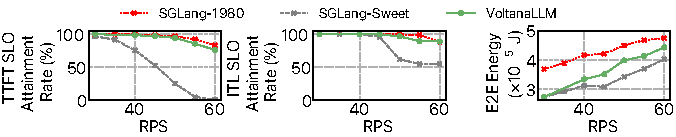
\includegraphics[width=\columnwidth]{figs/gh200_result.pdf}
    \caption{Latency SLO attainment and E2E energy consumption of \name on GH200, using Qwen3-32B and ShareGPT dataset.}
    % \jiahuan{@Junfeng, enlarge font size as \fref{fig:slo-sensitivity}, also apply its similiar format template}
    % \jiahuan{TODO: check decode result}
    \label{fig:exp-gh200}
\end{figure}


% \old{

% \jiahuan{move to \appref{subsubsec:pd-variation}}

% \noindent
% \textbf{What happens in varying the P/D throughput demand ratio?}
% \label{subsubsec:ablation-pd-ratio}
% As discussed in \sref{subsec:temporal-variation}, the temporal variation of P/D throughput demand ratio requires phase-specific frequency control.
% However, evaluating the whole Azure LLM Inference Trace dataset incurs significant GPU cost and time given it only shows fluctuation on the scale of hours.
% Hence, we use a synthetic dataset with P/D demand ratio fluctuating in 5 minutes. \fref{fig:ablation-pd-ratio} shows the evaluation results with LLaMA-3.1-8B using the same configuration in \sref{subsec:main-result}.


% The results shown in \tref{tab:ablation-pd-ratio} confirm the adaptiveness of \name.
% It can still maintain comparable SLO attainment rates to SGLang at maximum frequency, while obtain significant energy savings.
% \fref{fig:ablation-pd-ratio} shows the frequency dynamics.
% When prefill throughput demand is high, the prefill instance operates at a higher frequency,, while the decode instance remains at a low frequency.
% Conversely, when decode throughput demand is high, their roles reverse, shows highly adaptiveness.
% % Consequently, 
% % \jiahuan{TODO}

% % \jiahuan{TODO: report energy SLO}



% \begin{table}[!ht]
%     \centering 
%     % \small
%     \caption{Performance and energy under a synthetic workload with varying P/D demand ratios. TSAR/ISAR refers to TTFT/ITL SLO attainment rate. \jiahuan{TODO: redraw as a bar figure}}
%     \label{tab:ablation-pd-ratio}
%     \begin{tabular}{c|ccccccc}
%         \hline
%         \textbf{Metrics} & TSAR (\%) & ISAR (\%) &  Energy (J) \\
%         \hline
%         \textbf{\name} &96.05 &  91.74 & 289409\\
%         \textbf{SGLang (1005 MHz)} &77.86 & 36.78 &  257768 \\
%         \textbf{SGLang (1410 MHz)} &97.85 & 88.92 & 405340\\
%         \hline
%     \end{tabular}
% \end{table}

% \begin{figure}[!ht]
%     \centering
%     \begin{subfigure}[t]{0.42\columnwidth}
%         \centering
%         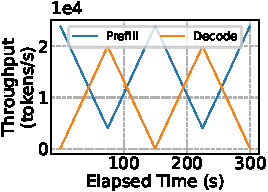
\includegraphics[width=\linewidth]{figs/ablation-pd-ratio-b.pdf}
%     \end{subfigure}
%     \hfill
%     \begin{subfigure}[t]{0.53\columnwidth}
%         \centering
%         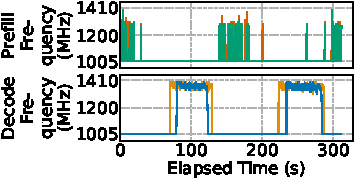
\includegraphics[width=\linewidth]{figs/ablation-pd-ratio-a.pdf}
%     \end{subfigure}
%     \caption{Left : P/D throughput with our synthetic dataset. Right : Frequency dynamics of all instances in \name. \jiahuan{to remove}}
%     \label{fig:ablation-pd-ratio}
% \end{figure}


% }